\documentclass[12pt]{article}

% Packages for better formatting
\usepackage{amsmath}  % For math symbols
\usepackage{amssymb}  % For additional math symbols
\usepackage{graphicx}
\usepackage{float}

\setlength{\parindent}{0pt}  % Turn off indentation globally

\DeclareMathOperator*{\argmin}{argmin}
\DeclareMathOperator*{\argmax}{argmax}

\title{Exercise solutions for Reinforcement Learning: An Introduction [2nd Edition]}
\author{Mátyás Pólya}
\date{\today}

\begin{document}

\maketitle

% Include exercise files
\section*{Chapter 1}

\textbf{Exercise 1.1: Self-Play} \\
Suppose, instead of playing against a random opponent, the
reinforcement learning algorithm described above played against itself, with both sides
learning. What do you think would happen in this case? Would it learn a different policy
for selecting moves? \\

\textbf{Solution:}
\begin{itemize}
    \item Early games would be random and unstructured.
    \item Over time, the agent would improve by reinforcing winning moves and avoiding losing ones.
    \item Eventually, the agent would converge toward optimal play, leading to most games ending in a draw.
    \item The RL agent would effectively learn to play tic-tac-toe perfectly, unable to lose but also unable to win against a similarly skilled opponent (itself).
  \end{itemize}

\textbf{Exercise 1.2 Symmetries} \\
Many tic-tac-toe positions appear different but are really
the same because of symmetries. How might we amend the learning process described
above to take advantage of this? In what ways would this change improve the learning
process? Now think again. Suppose the opponent did not take advantage of symmetries.
In that case, should we? Is it true, then, that symmetrically equivalent positions should
necessarily have the same value?\\

\textbf{Solution:}
\begin{itemize}
    \item Rather than treating each possible board configuration as unique, the RL agent should group board positions that are equivalent under symmetry. This would reduce the number of unique states the agent needs to learn/investigate.
    \item No, we shouldn't exploit symmetries if the opponent doesn't exploit them either. If the opponent has a policy that behaves differently at states that are symmetric to each other, then the agent couldn't expoit this if it treated symmetric states the same. In this case symmetrically equivalent positions should not have the same value.
  \end{itemize}

\textbf{Exercise 1.3 Greedy Play} \\
Suppose the reinforcement learning player was greedy, that is,
it always played the move that brought it to the position that it rated the best. Might it learn to play better, or worse, than a nongreedy player? What problems might occur? \\

\textbf{Solution:}
\begin{itemize}
    \item Case 1, The opponent is deterministic (always plays the same move at a certain state):\\
    In the beginnig, all of the non-winning states have a 50\% rating, so the greedy player would choose a random move. If this move leads to winning, its estimate increases, so in the following rounds the agent will choose it again and again. If it leads to losing, then its estimate decreases, so the agent will choose another move in the following rounds. This way the agent will find a set of steps that will always lead to winning (if they exist).
    \item Case 2, The opponent is non-deterministic:\\
    Suppose at first try the agent finds a set of steps which always produce an estimate that is $>50\%$. The greedy agent will always choose these steps (the others were initialized at 50\%), but there might be a set of steps that achieve better winrate. In this case there is no guarantee that the agent finds the best policy.\\
    (This is a special case, the winrate can be arbitrarily small)  
  \end{itemize}

\textbf{Exercise 1.4 Learning from Exploration} \\
Suppose learning updates occurred after all
moves, including exploratory moves. If the step-size parameter is appropriately reduced
over time (but not the tendency to explore), then the state values would converge to
a different set of probabilities. What (conceptually) are the two sets of probabilities
computed when we do, and when we do not, learn from exploratory moves? Assuming
that we do continue to make exploratory moves, which set of probabilities might be better
to learn? Which would result in more wins?\\

\textbf{Solution:}
\begin{itemize}
    \item If we don't update after exploratory moves: the value is the probability that a greedy agent wins from that state.
    \item If we update after exploratory moves: the value is the probability that an agent that is prone to explore wins from that state.
    \item If we continue to explore, then we should include the exploratory moves into the updates.
\end{itemize}

\textbf{Exercise 1.5 Other Improvements} \\
Can you think of other ways to improve the reinforcement learning player? Can you think of any better way to solve the tic-tac-toe problem
as posed?

\textbf{Solution:}
\begin{itemize}
    \item Incorporate domain knowledge (Heuristics and Rules): e.g. always take center.
    \item Use of Value Function Approximation: use a neural network or other function approximator to estimate the value function.
\end{itemize}
\section*{Chapter 2}

\textbf{Exercise 2.1} \\
In $\varepsilon$-greedy action selection, for the case of two actions and $\varepsilon = 0.5$, what is
the probability that the greedy action is selected? 

\textbf{Solution:} \\
$P(\text{greedy action is selected}) = P(\text{greedy action is selected} \mid \text{exploratory step}) \cdot P(\text{exploratory step}) +
 P(\text{greedy action is selected} \mid \text{non-exploratory step}) \cdot P(\text{non-exploratory step}) = 0.5 \cdot 0.5 + 1 \cdot 0.5 = 0.75$.\\


\textbf{Exercise 2.2: Bandit example} \\
Consider a $k$-armed bandit problem with $k = 4$ actions,
denoted 1, 2, 3, and 4. Consider applying to this problem a bandit algorithm using
$\varepsilon$-greedy action selection, sample-average action-value estimates, and initial estimates
of $Q_1(a) = 0$, for all $a$. Suppose the initial sequence of actions and rewards is $A_1 = 1$,
$R_1 = 1$, $A_2 = 2$, $R_2 = 1$, $A_3 = 2$, $R_3 = 2$, $A_4 = 2$, $R_4 = 2$, $A_5 = 3$, $R_5 = 0$. On some
of these time steps the $\varepsilon$ case may have occurred, causing an action to be selected at
random. On which time steps did this definitely occur? On which time steps could this
possibly have occurred?\\

\textbf{Solution:}

\begin{center}
    \begin{tabular}{|c|c|c|c|c|c|c|}
    \hline
        $t=$  & 0 & 1 & 2 & 3  & 4   & 5   \\ \hline 
    $Q_t(1)$ & 0  & \textbf{1}  & 1  & 1   & 1    & 1    \\ 
    $Q_t(2)$ & 0  & 0  & \textbf{1}  & \textbf{1.5} & \textbf{1.67} & 1.67 \\ 
    $Q_t(3)$ & 0  & 0  & 0  & 0   & 0    & \textbf{0}    \\ 
    $Q_t(4)$ & 0  & 0  & 0  & 0   & 0    & 0    \\ \hline
    \end{tabular}
\end{center}

\begin{itemize}
    \item $\varepsilon$ case definitely occured at $t \in \{2,5\}$
    \item It may have occured at any other time, too, just by chance the agent may have choosen the greedy step
\end{itemize} 

\textbf{Exercise 2.3} \\
In the comparison shown in Figure 2.2, which method will perform best in
the long run in terms of cumulative reward and probability of selecting the best action?
How much better will it be? Express your answer quantitatively.\\

\textbf{Solution:}\\
As $t \to \infty$ we have $Q_t(a) \to q_*(a)$ for all $a$. The agent with $\varepsilon=0.1$ will choose the correct action only $90\%$ of the time, while the agent with $\varepsilon=0.01$ will choose it $99\%$ of the time.\\

\textbf{Exercise 2.4} \\
If the step-size parameters, $a_n$, are not constant, then the estimate $Q_n$ is
a weighted average of previously received rewards with a weighting different from that
given by (2.6). What is the weighting on each prior reward for the general case, analogous
to (2.6), in terms of the sequence of step-size parameters?\\

\textbf{Solution:}\\
\begin{equation}
    \begin{aligned}
        Q_{n+1} &= Q_n + \alpha_n \left[ R_n - Q_n \right] \\
        &= \alpha_n  R_n + (1-\alpha_n) Q_n \\
        &= \alpha_n  R_n + (1-\alpha_n) \left[ \alpha_{n-1}  R_{n-1} + (1-\alpha_{n-1}) Q_{n-1} \right] \\
        &= \alpha_n  R_n + (1-\alpha_n) \alpha_{n-1}  R_{n-1} + (1-\alpha_n) (1-\alpha_{n-1}) Q_{n-1} \\
        &= \left( \prod_{i=1}^{n} (1-\alpha_i) \right) Q_1 + \sum_{i=1}^{n} \alpha_i R_i \prod_{k=i+1}^{n} (1-\alpha_k) 
\end{aligned}
\end{equation}
\\

\textbf{Exercise 2.5 (programming)} \\
 Design and conduct an experiment to demonstrate the
difficulties that sample-average methods have for nonstationary problems. Use a modified
version of the 10-armed testbed in which all the $q_*(a)$ start out equal and then take
independent random walks (say by adding a normally distributed increment with mean 0
and standard deviation 0.01 to all the $q_*(a)$ on each step). Prepare plots like Figure 2.2
for an action-value method using sample averages, incrementally computed, and another
action-value method using a constant step-size parameter, $\alpha = 0.1$. Use $\varepsilon = 0.1$ and
longer runs, say of 10,000 steps. \\

\textbf{Solution:}\\
See the notebook. \\
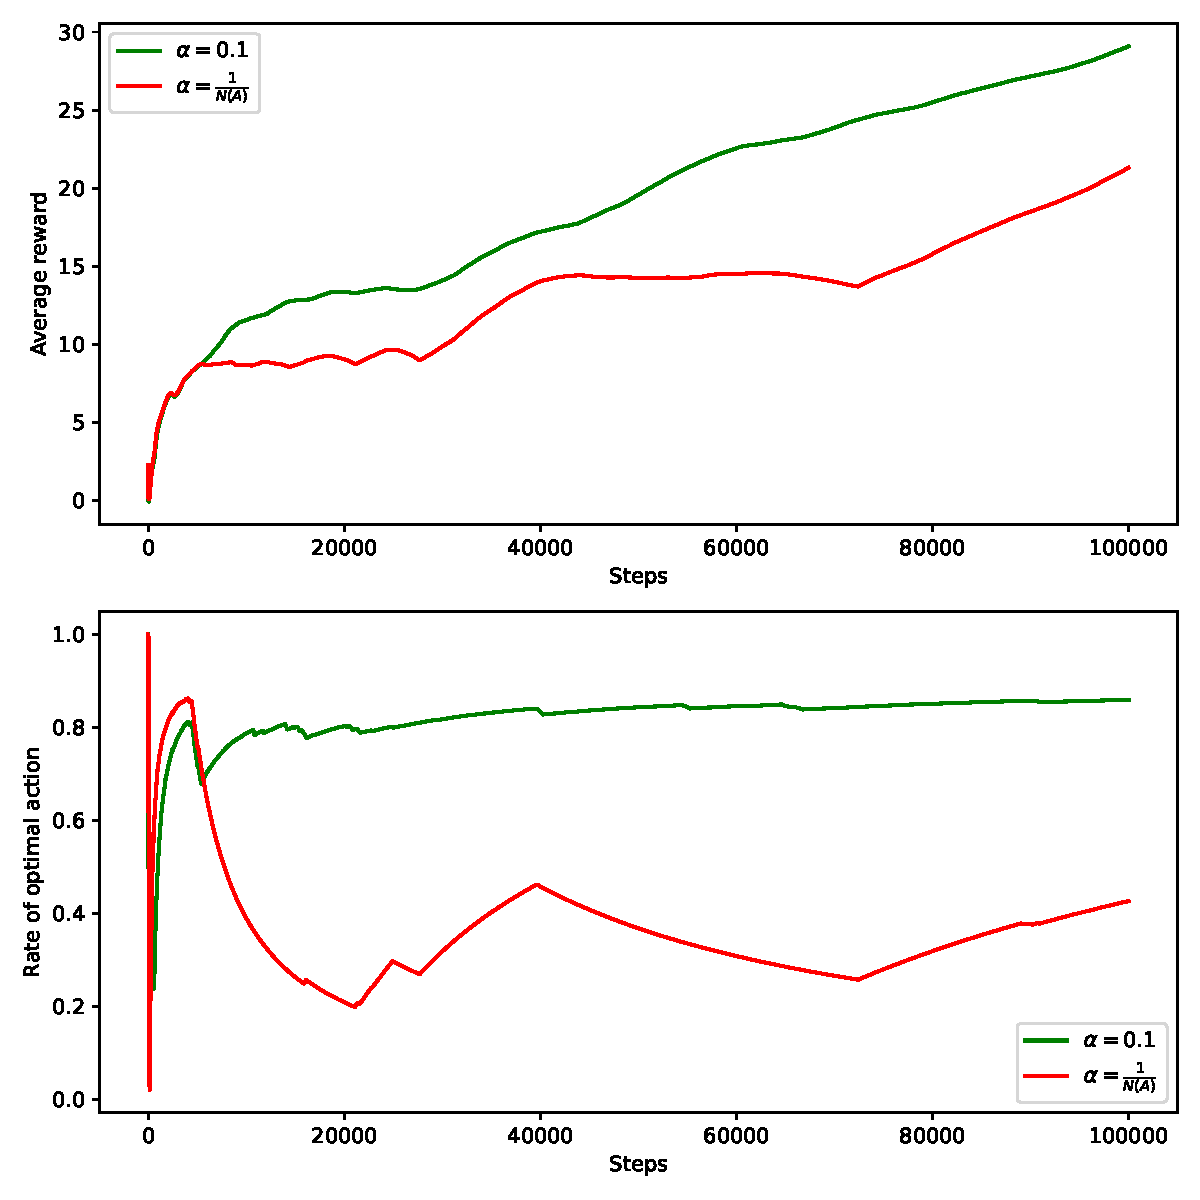
\includegraphics[width=\textwidth, angle=0]{chapters_latex/figures/ex_02_05.pdf}


\textbf{Exercise 2.6: Mysterious Spikes} \\
The results shown in Figure 2.3 should be quite reliable
because they are averages over 2000 individual, randomly chosen 10-armed bandit tasks.
Why, then, are there oscillations and spikes in the early part of the curve for the optimistic
method? In other words, what might make this method perform particularly better or
worse, on average, on particular early steps?\\

\textbf{Solution:}\\
The agent might choose the optimal action correctly, then through chance it could receive high rewards initially, so it will choose it many times, thus increasing the \% Optimal rate. After a while, again by chance, its estimate of the reward could decrease, so it would choose another suboptimal action, and the \% Optimal action would decrease. \\


\textbf{Exercise 2.7: Unbiased Constant-Step-Size Trick} \\
In most of this chapter we have used
sample averages to estimate action values because sample averages do not produce the
initial bias that constant step sizes do (see the analysis leading to (2.6)). However, sample
averages are not a completely satisfactory solution because they may perform poorly
on nonstationary problems. Is it possible to avoid the bias of constant step sizes while
retaining their advantages on nonstationary problems? One way is to use a step size of
\begin{equation}
    \beta_t \doteq \alpha / \bar{o}_t,
\end{equation}
where $\alpha > 0$ is a conventional constant step size and $\bar{o}_t$ is a trace of one that starts at 0:
\begin{equation}
    \bar{o}_{t+1} = \bar{o}_t + \alpha (1 - \bar{o}_t)
\end{equation}
for $t \geq 1$ and with $\bar{o}_1 \doteq \alpha$. \\

Carry out an analysis like that in (2.6) to show that $Q_n$ is an exponential recency-weighted average without initial bias.\\

\textbf{Solution:}\\

$\bar{o}_{t+1} = \bar{o}_t + \alpha (1 - \bar{o}_t) = \bar{o}_t(1-\alpha) + \alpha $\\

\begin{equation}
    \begin{aligned}
        \bar{o}_{1} &= \alpha \\
        \bar{o}_{2} &= \alpha + \alpha(1- \alpha) = 2\alpha - \alpha^2 \\
        \bar{o}_{t} &= \sum_{i=1}^{t} \alpha (1-\alpha)^{t-i}\\
        &=1-\left(1-\alpha\right)^{t}\\
    \end{aligned}
\end{equation}

\begin{equation}
    \begin{aligned}
        Q_{n+1} &= Q_n + \beta_n \left[ R_n - Q_n \right] \\
        &= Q_n + \frac{\alpha}{1-\left(1-\alpha\right)^{n}} \left[ R_n - Q_n \right] \\
        %&= \left( \prod_{i=1}^{n} (1-\beta_i) \right) Q_1 + \sum_{i=1}^{n} \beta_i R_i \prod_{k=i+1}^{n} (1-\beta_k) \\ 
        %&= \left( \prod_{i=1}^{n} (1-\alpha / \bar{o}_i) \right) Q_1 + \sum_{i=1}^{n} \alpha / \bar{o}_i R_i \prod_{k=i+1}^{n} (1-\alpha / \bar{o}_k) \\
    \end{aligned}
\end{equation}

The $\beta_n$ is decreasing, so it is recency-weighted. The contribution of the initial estimate $Q_1$ diminishes to zero as $t$ increases, the system effectively forgets the initial bias after a sufficient number of updates.\\

\textbf{Exercise 2.8: UCB Spikes}\\
In Figure 2.4 the UCB algorithm shows a distinct spike
in performance on the 11th step. Why is this? Note that for your answer to be fully
satisfactory it must explain both why the reward increases on the 11th step and why it
decreases on the subsequent steps. Hint: If $c = 1$, then the spike is less prominent.\\

\textbf{Solution:}

At the timesteps $t \leq 10$ there is always an action $a$ for which $N_t(a) = 0$, so the agent will always choose that action. After the 10th step the agent will choose greedily so the average reward increases. After some timesteps the uncertainty term of some other action overtakes the previously chosen action, and the agent starts to explore again, so the average reward decreases.\\

\textbf{Exercise 2.9}\\
Show that in the case of two actions, the soft-max distribution is the same
as that given by the logistic, or sigmoid, function often used in statistics and artificial
neural networks.\\

\textbf{Solution:}\\

\begin{equation}
    \begin{aligned}
        P(A_t = 1) &= \frac{e^{H_t(1)}}{\sum_{b=1}^{2} e^{H_t(b)}} = \frac{e^{H_t(1)}}{e^{H_t(1)} + e^{H_t(0)}} = \frac{1}{1 + e^{-(H_t(1)-H_t(0))}} \\
        &= \sigma(H_t(1)-H_t(0))
    \end{aligned}
\end{equation}


\textbf{Exercise 2.10}\\
Suppose you face a 2-armed bandit task whose true action values change
randomly from time step to time step. Specifically, suppose that, for any time step,
the true values of actions 1 and 2 are respectively 10 and 20 with probability 0.5 (case
A), and 90 and 80 with probability 0.5 (case B). If you are not able to tell which case
you face at any step, what is the best expected reward you can achieve and how should
you behave to achieve it? Now suppose that on each step you are told whether you are
facing case A or case B (although you still don't know the true action values). This is an
associative search task. What is the best expected reward you can achieve in this task,
and how should you behave to achieve it?\\

\textbf{Solution}\\
If we can't differentiate the 2 cases:\\
Suppose the agent chooses action 1 with probability $p$. Then the expected reward is:
\begin{equation}
    \begin{aligned}
    \mathbb{E}[R] &= P(A) \cdot \left( p R_A(1) + (1-p)  R_A(2) \right) + 
                    P(B) \cdot \left( p R_B(1) + (1-p)  R_B(2) \right)\\
        &= 0.5 (10p + 20(1-p)) + 0.5 (90p + 80(1-p)) \\
        &= 50
    \end{aligned}
\end{equation}

If we \emph{can} differentiate the 2 cases:\\
We want to maximize the reward, so in case A the agent should choose action 2 and in case B it should choose action 1.   
\begin{equation}
    \begin{aligned}
    \mathbb{E}[R] &= P(A) \cdot R_A(2) + P(B) \cdot R_B(1) \\
        &= 0.5 \cdot 20 + 0.5 \cdot 90 \\
        &= 55
    \end{aligned}
\end{equation}


\textbf{Exercise 2.11 (programming)}\\
Make a figure analogous to Figure 2.6 for the nonstationary
case outlined in Exercise 2.5. Include the constant-step-size $\varepsilon$-greedy algorithm with
$\alpha = 0.1$. Use runs of 200,000 steps and, as a performance measure for each algorithm and
parameter setting, use the average reward over the last 100,000 steps.\\

\textbf{Solution:}\\
See the notebook. \\
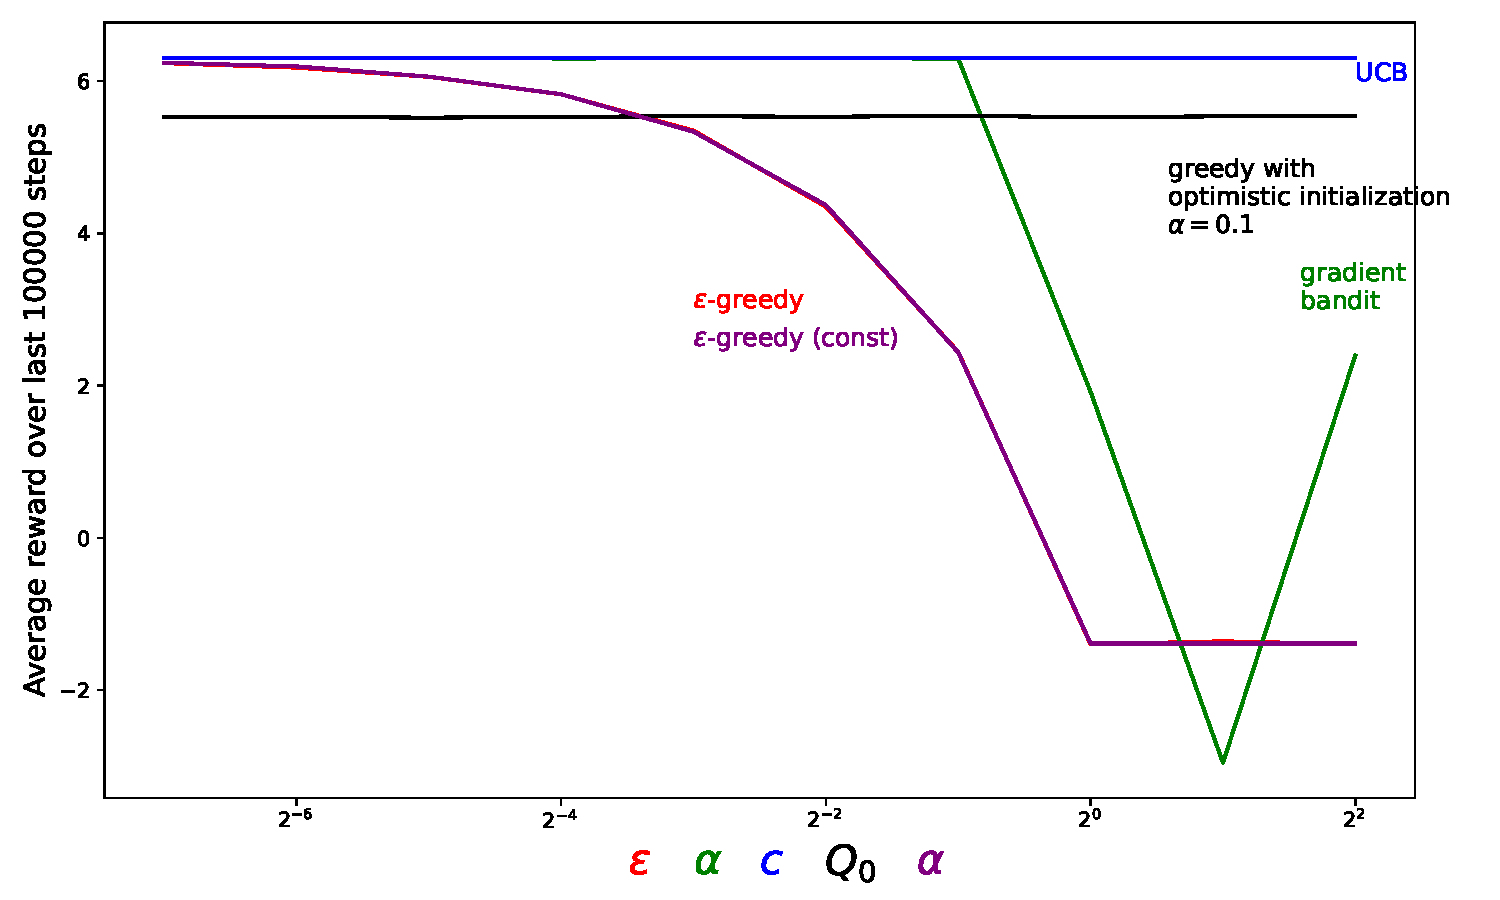
\includegraphics[width=\textwidth, angle=0]{chapters_latex/figures/ex_02_11_reward.pdf}
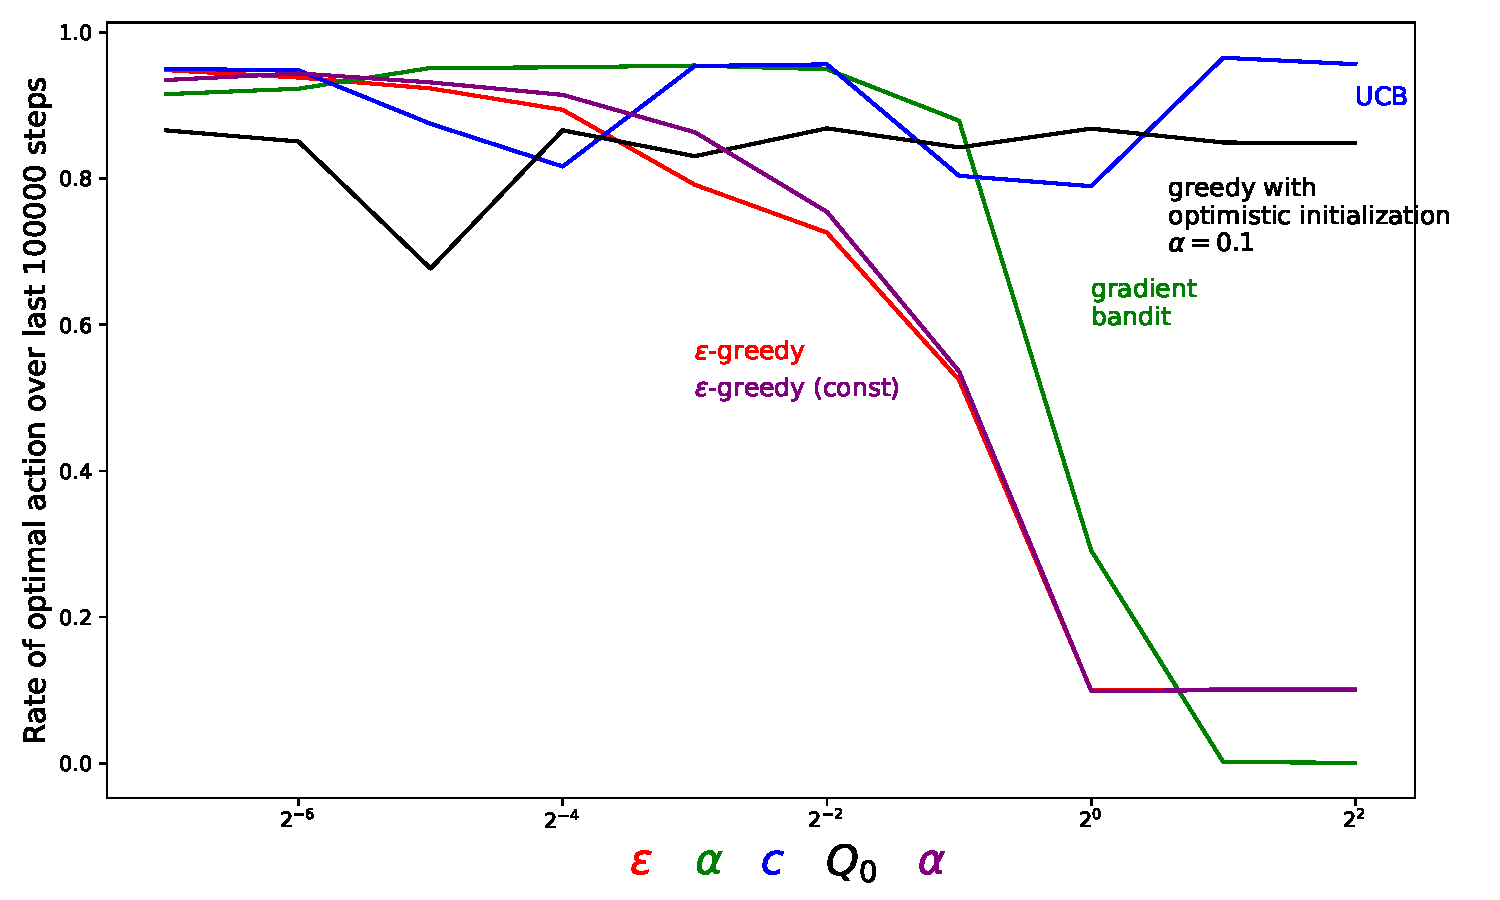
\includegraphics[width=\textwidth, angle=0]{chapters_latex/figures/ex_02_11_rate.pdf}

\section*{Chapter 3}

\subsection*{Exercise 3.1}
Devise three example tasks of your own that fit into the MDP framework,
identifying for each its states, actions, and rewards. Make the three examples as different
from each other as possible. The framework is abstract and flexible and can be applied in
many different ways. Stretch its limits in some way in at least one of your examples.

\subsubsection*{Solution:}
Example 1: Chess Player Program\\
Task Description: A chess-playing program aims to play chess in a way that conceals its identity as a non-human player.

\begin{itemize}
    \item \textbf{States (S):}
    \begin{itemize}
        \item Current board position (the arrangement of pieces).
        \item Time remaining for each player.
        \item Opponent's previous move history.
    \end{itemize}
    
    \item \textbf{Actions (A):}
    \begin{itemize}
        \item Make a legal move
        \item Pause (to simulate human behavior, potentially to analyze).
        \item Offer a draw or resignation.
    \end{itemize}
    
    \item \textbf{Rewards (R):}
    \begin{itemize}
        \item +1 for winning the game.
        \item -1 for drawing or losing.
        \item -0.01 for making moves that are too optimal, which might reveal the program's identity (e.g., moving in a way that a human wouldn't).
        \item +0.01 for making "human-like" moves (less optimal but more deceptive).
    \end{itemize}
\end{itemize}

Example 2: Person Taking an IQ Test\\
Task Description: A person takes an IQ test with the goal of maximizing their score.

\begin{itemize}
    \item \textbf{States (S):}
    \begin{itemize}
        \item Current question number.
        \item The question itself.
        \item Time left for the test.
    \end{itemize}
    
    \item \textbf{Actions (A):}
    \begin{itemize}
        \item Answer the question (select one of multiple-choice options).
        \item Think.
        \item Skip the question.
    \end{itemize}
    
    \item \textbf{Rewards (R):}
    \begin{itemize}
        \item +1 for a correct answer.
        \item 0 for a skipped question.
        \item -1 for an incorrect answer.
    \end{itemize}
\end{itemize}

Example 3: Elevator Control System\\
Task Description: An elevator system optimizes its operation to minimize wait times and maximize efficiency in a multi-story building.

\begin{itemize}
    \item \textbf{States (S):}
    \begin{itemize}
        \item Current floor of the elevator.
        \item Status of the elevator (moving up, moving down, idle).
        \item Status of the door (open, closed)
        \item Floors where people wish to go up.
        \item Floors where people wish to go down.
        \item Current load (number of passengers in the elevator based on weight).
        \item Buttons pressed (which floors the passengers in the elevator wish to go to).
    \end{itemize}
    
    \item \textbf{Actions (A):}
    \begin{itemize}
        \item Move up.
        \item Move down.
        \item Open doors.
        \item Close doors.
        \item Wait on the current floor.
    \end{itemize}
    
    \item \textbf{Rewards (R):}
    \begin{itemize}
        \item -1 for each second the passengers spend waiting.
        \item -1 for unnecessary movements (e.g., moving to a floor with no waiting passengers).
    \end{itemize}
\end{itemize}


\subsection*{Exercise 3.2}
Is the MDP framework adequate to usefully represent all goal-directed learning tasks? Can you think of any clear exceptions?

\subsubsection*{Solution:}
There are situations where the MDP framework is not adequate. 
\begin{itemize}
    \item Continous action spaces
    \item Non-Markovian environments
    \item High-Dimensional state spaces
\end{itemize}

Example: self-driving for cars have continous action spaces (steering the wheel, rate of acceleration) and high-dimensional state spaces (images of the environment).

\subsection*{Exercise 3.3}
Consider the problem of driving. You could define the actions in terms of
the accelerator, steering wheel, and brake, that is, where your body meets the machine.
Or you could define them farther out—say, where the rubber meets the road, considering
your actions to be tire torques. Or you could define them farther in—say, where your
brain meets your body, the actions being muscle twitches to control your limbs. Or you
could go to a really high level and say that your actions are your choices of where to drive.
What is the right level, the right place to draw the line between agent and environment?
On what basis is one location of the line to be preferred over another? Is there any
fundamental reason for preferring one location over another, or is it a free choice?

\subsubsection*{Solution:} 
The right place to draw the line between agent and environment is highly dependant on the problem we are modeling/trying to solve. If we want to create a route finding algorithm, then the highest level of choice would be ideal, but if we want to look at the problem in a neuroscientific way, then the brain and muscle option would be fine.\\
There is no fundamental reason for preferring one location over another, it is only good for using the advantages of abstraction.


\subsection*{Exercise 3.4}
Give a table analogous to that in Example 3.3, but for $p(s', r |s, a)$ . It
should have columns for $s$, $a$, $s'$, $r$, and $p(s', r |s, a)$ , and a row for every 4-tuple for which
$p(s', r |s, a)  > 0$.

\subsubsection*{Solution:}

\begin{table}[h!]
    \centering
    \begin{tabular}{ll|ll|c}
        $s$  & $a$      & $s'$ & $r$                 & $p(s', r |s, a)$ \\ \hline
        high & search   & high & $r_{\text{search}}$ & $\alpha$         \\
        high & search   & low  & $r_{\text{search}}$ & $1 - \alpha$     \\
        low  & search   & high & -3                  & $1 - \beta$      \\
        low  & search   & low  & $r_{\text{search}}$ & $\beta$          \\
        high & wait     & high & $r_{\text{wait}}$   & 1                \\
        low  & wait     & low  & $r_{\text{wait}}$   & 1                \\
        low  & recharge & high & 0                   & 1               
    \end{tabular}
\end{table}


\subsection*{Exercise 3.5}
The equations in Section 3.1 are for the continuing case and need to be
modified (very slightly) to apply to episodic tasks. Show that you know the modifications
needed by giving the modified version of (3.3).

\subsubsection*{Solution:}
The original equation:
\[
\sum_{s' \in S} \sum_{r \in R} P(s', r \mid s, a) = 1, \quad \forall s \in S, \forall a \in A(s)
\]

This would exclude the terminal states $S^+ \setminus S$, so we wouldn't count the cases where a state goes from non-terminal to a terminal state.

The modified equation:
\[
\sum_{s' \in S^+} \sum_{r \in R} P(s', r \mid s, a) = 1, \quad \forall s \in S^+, \forall a \in A(s)
\]


\subsection*{Exercise 3.6}
Suppose you treated pole-balancing as an episodic task but also used
discounting, with all rewards zero except for  1 upon failure. What then would the
return be at each time? How does this return differ from that in the discounted, continuing
formulation of this task?

\subsubsection*{Solution:}

\[
G_t = \sum_{k=0}^{T-t} \gamma^k r_{t+k+1} = 0 + 0 + 0 + \dots + -\gamma^{T-t} = -\gamma^{T-t}
\]

The reward in the discounted, continuing formulation:

\[
G_t = \sum_{k \in K} -\gamma^{k-t}
\]

Where $K$ is the number of time steps before failure (as well as to the times of later failures).


\subsection*{Exercise 3.7} Imagine that you are designing a robot to run a maze. You decide to give it a
reward of +1 for escaping from the maze and a reward of zero at all other times. The task
seems to break down naturally into episodes—the successive runs through the maze—so
you decide to treat it as an episodic task, where the goal is to maximize expected total
reward (3.7). After running the learning agent for a while, you find that it is showing
no improvement in escaping from the maze. What is going wrong? Have you effectively
communicated to the agent what you want it to achieve?

\subsubsection*{Solution:}

The agent receives +1 reward regardless of the timesteps it takes it to leave the maze. Because of this, it can't distinguish a good policy from a bad one.

\subsection*{Exercise 3.8}
Suppose $\gamma = 0.5$ and the following sequence of rewards is received $R_1 = -1$, $R_2 = 2$, $R_3 = 6$, $R_4 = 3$, and $R_5 = 2$, with $T = 5$. What are $G_0$, $G_1$, $\dots$, $G_5$? Hint:
Work backwards.

\subsubsection*{Solution:}

\begin{equation}
    \begin{aligned}
        G_t &= R_{t+1} + \gamma G_{t+1} \\
        G_5 &= 0 \\
        G_4 &= 2 + 0.5 \cdot 0 = 2 \\
        G_3 &= 3 + 0.5 \cdot 2 = 4 \\
        G_2 &= 6 + 0.5 \cdot 4 = 8 \\
        G_1 &= 2 + 0.5 \cdot 8 = 6 \\
        G_0 &= -1 + 0.5 \cdot 6 = 2 \\
    \end{aligned}
\end{equation}


\subsection*{Exercise 3.9}
Suppose  $\gamma = 0.9$ and the reward sequence is $R_1 = 2$ followed by an infinite
sequence of 7s. What are $G_1$ and $G_0$? 

\subsubsection*{Solution:}

\[
G_0 = 2 + \sum_{k = 1}^{\infty} 0.9^k \cdot 7  = 2 + \frac{0.9 \cdot 7}{1-0.9} = 65
\]

\[
G_1 = \sum_{k = 0}^{\infty} 0.9^k \cdot 7 = \frac{7}{1-0.9} = 70
\]

\subsection*{Exercise 3.10}
Prove the second equality in (3.10).

\subsubsection*{Solution:}

The equality in question:

\[
\sum_{k = 0}^{\infty} \gamma^k = \frac{1}{1-\gamma}
\]

Proof:

\begin{align*}
    \sum_{k = 0}^{\infty} \gamma^k &= 1 + \gamma + \gamma^2 + \gamma^3 + \dots \\
    &= 1 + \gamma (1 + \gamma + \gamma^2  + \dots) \\
    &= 1 + \gamma \sum_{k = 0}^{\infty} \gamma^k
\end{align*}

\[
(1 - \gamma)\sum_{k = 0}^{\infty} \gamma^k = 1
\]

\[
\sum_{k = 0}^{\infty} \gamma^k = \frac{1}{1 - \gamma}
\]

\subsection*{Exercise 3.10}
If the current state is $S_t$, and actions are selected according to a stochastic
policy $\pi$, then what is the expectation of $R_{t+1}$ in terms of $\pi$ and the four-argument
function $p$ (3.2)?

\subsubsection*{Solution:}

\[
    \mathbb{E}_{\pi} \left[R_{t+1} | S_t = s \right] = \sum_r r  \sum_{s', a} \pi(a|s) p(s', r | s, a)
\]

\subsection*{Exercise 3.12}
Give an equation for $v_\pi$ in terms of $q_\pi$ and $\pi$.

\subsubsection*{Solution:}
\begin{align*}
    v_\pi(s)&=\mathbb{E}_{\pi} \left[G_{t+1} | S_t = s \right] \\
    &= \sum_a \mathbb{E}_{\pi} \left[G_{t+1} | S_t = s, A_t = a \right] \pi(a|s)\\
    &= \sum_a q_\pi(s,a) \pi(a|s)
\end{align*}

\subsection*{Exercise 3.13}
Give an equation for $q_\pi$ in terms of $v_\pi$ and the four-argument $p$.

\subsubsection*{Solution:}

\begin{align*}
    q_\pi(s, a) &= \mathbb{E}_{\pi} \left[G_{t+1} | S_t = s, A_t = a \right] \\
    &= \sum_{s',r} p(s', r | s, a) (r + \gamma \mathbb{E}_{\pi} \left[G_{t+2} | S_{t+1} = s' \right]) \\
    &= \sum_{s',r} p(s', r | s, a) (r + \gamma v_\pi(s'))
\end{align*}


\subsection*{Exercise 3.14}
The Bellman equation (3.14) must hold for each state for the value function
$v_\pi$ shown in Figure 3.2 (right) of Example 3.5. Show numerically that this equation holds
for the center state, valued at $+0.7$, with respect to its four neighboring states, valued at
$+2.3$, $+0.4$,  $-0.4$, and $+0.7$. (These numbers are accurate only to one decimal place.)

\subsubsection*{Solution:}

\begin{align*}
    v_\pi(s) &= \sum_a \pi(a|s) \sum_{s',r} p(s',r |s, a)\left[r + \gamma v_\pi(s')\right] \\
    &= 0.25 \cdot 0.9 \cdot (2.3 + 0.4 - 0.4 + 0.7) \\
    &= 0.675
\end{align*}

\subsection*{Exercise 3.15}
In the gridworld example, rewards are positive for goals, negative for
running into the edge of the world, and zero the rest of the time. Are the signs of these
rewards important, or only the intervals between them? Prove, using (3.8), that adding a
constant $c$ to all the rewards adds a constant, $v_c$, to the values of all states, and thus
does not affect the relative values of any states under any policies. What is $v_c$ in terms
of $c$ and $\gamma$? 

\subsubsection*{Solution:}
\begin{align*}
    G_t' &= \sum_{k=0}^{\infty}\gamma^k (R_{t+k+1}+c) \\
    &= \sum_{k=0}^{\infty}\gamma^k R_{t+k+1} + c \sum_{k=0}^{\infty}\gamma^k \\
    &= G_t + \frac{c}{1 - \gamma}
\end{align*}

\subsection*{Exercise 3.16}
Now consider adding a constant $c$ to all the rewards in an episodic task,
such as maze running. Would this have any effect, or would it leave the task unchanged
as in the continuing task above? Why or why not? Give an example.

\subsubsection*{Solution:}
This could have an adverse effect for the task. The maze running example could be formulated as the agent getting a -1 reward every timestep while still in the maze, and a 0 reward when reaching the exit. Adding a $c > 1$ constant to every reward would mean that the agent is incentivised to stay in the maze and avoid the exit.

\subsection*{Exercise 3.17}
What is the Bellman equation for action values, that
is, for $q_\pi$? It must give the action value $q_\pi(s,a)$ in terms of the action
values, $q_\pi(s',a')$, of possible successors to the state-action pair $(s,a)$.
Hint: The backup diagram to the right corresponds to this equation.
Show the sequence of equations analogous to (3.14), but for action
values.

\subsubsection*{Solution:}

\begin{align*}
    q_\pi(s, a) &= \mathbb{E}_{\pi} \left[G_{t+1} | S_t = s, A_t = a \right] \\
    &= \sum_{s',r} p(s', r | s, a) \left(r + \gamma \sum_{a'} \pi(a'|s') \mathbb{E}_{\pi} \left[G_{t+2} | S_{t+1} = s', A_{t+1} = a' \right]\right) \\
    &= \sum_{s',r} p(s', r | s, a) \left(r + \gamma \sum_{a'} \pi(a'|s') q_\pi(s',a')\right)
\end{align*}

\subsection*{Exercise 3.18}
The value of a state depends on the values of the actions possible in that
state and on how likely each action is to be taken under the current policy. We can
think of this in terms of a small backup diagram rooted at the state and considering each
possible action:

\begin{center}
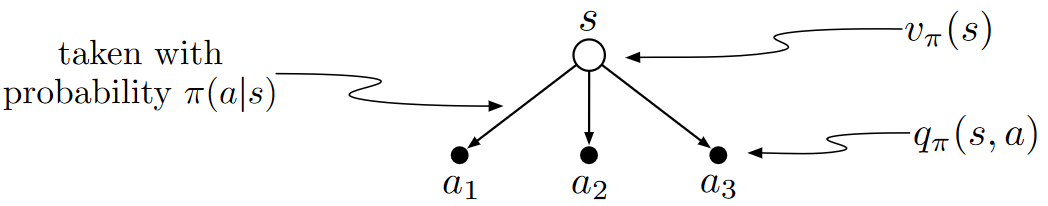
\includegraphics[width=0.8\textwidth]{chapters_latex/figures/ex_03_18.png}
\end{center}

Give the equation corresponding to this intuition and diagram for the value at the root
node, $v_\pi(s)$, in terms of the value at the expected leaf node, $q_\pi(s,a)$, given $S_t = s$. This
equation should include an expectation conditioned on following the policy, $\pi$. Then give
a second equation in which the expected value is written out explicitly in terms of $\pi(a|s)$
such that no expected value notation appears in the equation.

\subsubsection*{Solution:}

\[
    v_\pi(s)= \mathbb{E}_{\pi} \left[q_\pi(s,a) | S_t = s \right]
\]

\[
    v_\pi(s)= \sum_a \pi(a|s) q_\pi(s,a)
\]

\subsection*{Exercise 3.19} The value of an action, $q_\pi(s,a)$, depends on the expected next reward and
the expected sum of the remaining rewards. Again we can think of this in terms of a
small backup diagram, this one rooted at an action (state-action pair) and branching to
the possible next states:

\begin{center}
    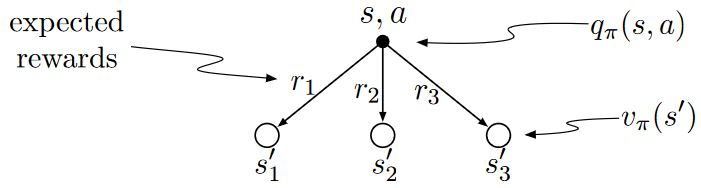
\includegraphics[width=0.6\textwidth]{chapters_latex/figures/ex_03_19.png}
\end{center}

Give the equation corresponding to this intuition and diagram for the action value,
$q_\pi(s,a)$, in terms of the expected next reward, $R_{t+1}$, and the expected next state value,
$v_\pi(S_{t+1})$, given that $S_t = s$ and $A_t = a$. This equation should include an expectation but
not one conditioned on following the policy. Then give a second equation, writing out the
expected value explicitly in terms of $p(s',r|s,a)$ defined by (3.2), such that no expected
value notation appears in the equation. 

\subsubsection*{Solution:}

\[
    q_\pi(s, a)= \mathbb{E} \left[R_{t+1} + \gamma v_\pi(S_{t+1}) | S_t = s, A_t = a \right]
\]

\[
    q_\pi(s, a)= \sum_{s',r} p(s',r|s,a) \left( r + \gamma v_\pi(s') \right)
\]


\subsection*{Exercise 3.20}
Draw or describe the optimal state-value function for the golf example.

\subsubsection*{Solution:}
Use the putter when on the green, use the driver in the other cases.
\begin{center}
    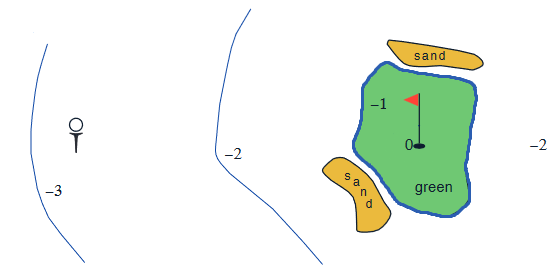
\includegraphics[width=0.6\textwidth]{chapters_latex/figures/ex_03_20.png}
\end{center}

\subsection*{Exercise 3.21} 
Draw or describe the contours of the optimal action-value function for putting, $q_*(s, \text{putter})$, for the golf example. 

\subsubsection*{Solution:}
$q_*(s, \text{putter})$ is equal to $1 + v_*(s')$ where $s'$ is the new location of the ball. If the ball arrives at the green, the next action should be using a putter, else the agent should use a driver.
\begin{center}
    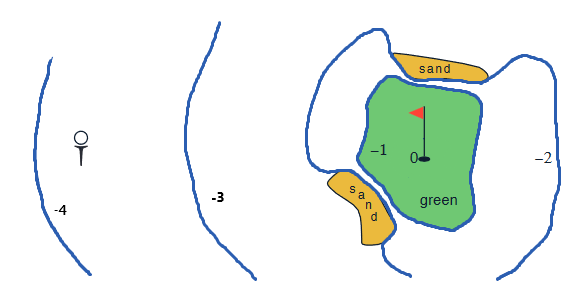
\includegraphics[width=0.6\textwidth]{chapters_latex/figures/ex_03_21.png}
\end{center}

\subsection*{Exercise 3.22}
Consider the continuing MDP shown to the
right. The only decision to be made is that in the top state,
where two actions are available, left and right. The numbers
show the rewards that are received deterministically after
each action. There are exactly two deterministic policies,
$\pi_\text{left}$ and $\pi_\text{right}$. What policy is optimal if  $\gamma = 0$? If  $\gamma = 0.9$?
If  $\gamma = 0.5$?
\begin{center}
    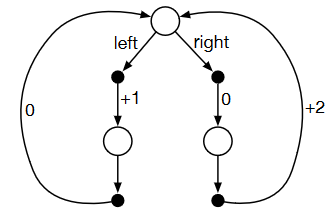
\includegraphics[width=0.6\textwidth]{chapters_latex/figures/ex_03_22.png}
\end{center}

\subsubsection*{Solution:}

After 2 actions the state will return to the original state, so $R_n = R_{n+2}$

\[
G_t = R_{t+1} + \gamma R_{t+2} + \gamma^2 G_t
\]

\[
(1 - \gamma^2) G = R_{t+1} + \gamma R_{t+2}
\]

\[
G_t = \frac{R_{t+1} + \gamma R_{t+2}}{1 - \gamma^2}
\]

$\pi_{\text{right}}$:   $G_t = \frac{2 \gamma}{1 - \gamma^2} $

$\pi_{\text{left}}$:   $G_t = \frac{1}{1 - \gamma^2} $

The optimal policy maximizes the value function, and because there is no stochasticity, $G_t = v_{\pi}(s)$.

If $(2\gamma > 1)$, going right is the optimal policy, while in the case of $(2\gamma < 1)$, going left is optimal.

For $(\gamma = 0)$: left is the optimal policy.

For $(\gamma = 0.9)$: right is the optimal policy.

For $(\gamma = 0.5)$: both policies are optimal.

\subsection*{Exercise 3.23}
Give the Bellman equation for $q_*$ for the recycling robot.

\subsubsection*{Solution:}

\begin{align*}
    q_*(\text{high}, \text{search}) &= r_\text{search} + \gamma \left( \alpha \max_a q_*(\text{high}, a) + (1 - \alpha) \max_a q_*(\text{low}, a) \right) \\
    q_*(\text{high}, \text{wait}) &= r_\text{wait} + \gamma \max_aq_*(\text{high}, a) \\
    q_*(\text{low}, \text{search}) &= \beta \left( r_\text{search} + \gamma  \max_a q_*(\text{low}, a) \right) \\
    &\quad + (1 - \beta) \left(-3 + \max_a q_*(\text{high}, a) \right) \\
    q_*(\text{low}, \text{wait}) &= r_\text{wait} + \gamma \max_aq_*(\text{low}, a) \\
    q_*(\text{low}, \text{recharge}) &= \gamma \max_aq_*(\text{high}, a)
\end{align*}

\subsection*{Exercise 3.24}
Figure 3.5 gives the optimal value of the best state of the gridworld as
24.4, to one decimal place. Use your knowledge of the optimal policy and (3.8) to express
this value symbolically, and then to compute it to three decimal places. 

\subsubsection*{Solution:}

\[
G_t = 10 + 0 + 0 + 0 + 0 + 0.9^5 \cdot G_t
\]
\[
G_t = \frac{10}{1-0.9^5} = 24.419
\]


\subsection*{Exercise 3.25}
Give an equation for $v_*$ in terms of $q_*$.

\subsubsection*{Solution:}

\[
v_*(s) = \max_a q_*(s,a)
\]

\subsection*{Exercise 3.26}
Give an equation for $q_*$ in terms of $v_*$ and the four-argument $p$.

\subsubsection*{Solution:}

\[
q_*(s,a) = \sum_{s', r} p(s', r |s, a)  \left( r + \gamma v_*(s') \right)
\]

\subsection*{Exercise 3.27}
Give an equation for $\pi_*$ in terms of $q_*$.

\subsubsection*{Solution:}

\[
\pi_*(a|s) =
    \begin{cases}
        1,  & \text{if } a = \argmax_a q_*(s,a)\\
        0,  & \text{else}
    \end{cases}
\]


\subsection*{Exercise 3.28}
Give an equation for $\pi_*$ in terms of $v_*$ and the four-argument $p$.

\subsubsection*{Solution:}

\[
\pi_*(a|s) =
    \begin{cases}
        1,  & \text{if } a = \argmax_a \sum_{s', r} p(s', r |s, a)  \left( r + \gamma v_*(s') \right)\\
        0,  & \text{else}
    \end{cases}
\]

\subsection*{Exercise 3.29}
Rewrite the four Bellman equations for the four value functions ($v_\pi$, $v_*$, $q_\pi$, $q_*$)
in terms of the three argument function $p$ (3.4) and the two-argument function $r$ (3.5).

\subsubsection*{Solution:}

\[
q_\pi(s,a) = r(s,a) + \gamma \sum_{s',a'} p(s'|s,a) \pi(a'|s') q _\pi(s',a')
\]

\[
    q_*(s,a) = r(s,a) + \gamma  \sum_{s'} p(s'|s,a) \max_{a'} \pi(a'|s') q _*(s',a')
\]

\[
    v_\pi(s) = \sum_a \pi(a|s) \left( r(s,a) + \gamma \sum_{s'} p(s'|s,a) v_\pi(s') \right) 
\]

\[
    v_*(s) = \max_a  r(s,a) + \gamma \sum_{s'} p(s'|s,a) v_*(s') 
\]
\section*{Chapter 4}

\subsection*{Exercise 4.1}

\subsubsection*{Solution:}
In Example 4.1, if $\pi$ is the equiprobable random policy, what is $q_\pi(11, \text{down})$?
What is $q_\pi(7, \text{down})$?

\[
q_\pi(11, \text{down}) = r + v_\pi(\text{end state}) = -1 + 0 = -1
\]

\[
q_\pi(7, \text{down}) = r + v_\pi(11) = -1 - 14 = -15
\]


\subsection*{Exercise 4.2}
In Example 4.1, suppose a new state 15 is added to the gridworld just below
state 13, and its actions, left, up, right, and down, take the agent to states 12, 13, 14,
and 15, respectively. Assume that the transitions from the original states are unchanged.
What, then, is $v_\pi(15)$ for the equiprobable random policy? Now suppose the dynamics of
state 13 are also changed, such that action down from state 13 takes the agent to the new
state 15. What is $v_\pi(15)$ for the equiprobable random policy in this case?

\subsubsection*{Solution:}
First case:
\[
v_\pi(15) = -1 + 0.25(v_\pi(12) + v_\pi(13) + v_\pi(14) + v_\pi(15))
\]

\[
v_\pi(15) = -\frac{4}{3} + \frac{1}{3}(v_\pi(12) + v_\pi(13) + v_\pi(14) ) = -\frac{4}{3} + \frac{1}{3}(-22 - 20 - 14) = -20
\]

Second case:

Using the iterative method with $v_\pi^1(15) = -20$.
\begin{align*}
v_\pi^1(13) &= -1 + 0.25(v_\pi(12) + v_\pi(9) + v_\pi(14) + v_\pi(15)) \\
&= -1 + 0.25(-22 - 20 - 14 - 20) = -20
\end{align*}

The $v(s)$ values didn't change, so the iterative algorithm can terminate here, $v_\pi(15) = -20$.

\subsection*{Exercise 4.3}
What are the equations analogous to (4.3), (4.4), and (4.5), but for action-
value functions instead of state-value functions?

\subsubsection*{Solution:}

\begin{align*}
    q_\pi(s, a) &= \mathbb{E} \left[R_{t+1} + \gamma \sum_{a'} \pi(a' \mid S_{t+1}) q_\pi(S_{t+1}, a') \middle| S_t = s, A_t = a \right] \\
    &= \sum_{s',r} p(s', r \mid s, a) \left(r + \gamma \sum_{a'} \pi(a'\mid s') q_\pi(s', a') \right)
\end{align*}

\[
    q_{k+1}(s, a) = \sum_{s',r} p(s', r \mid s, a) \left(r + \gamma \sum_{a'} \pi(a' \mid s') q_{k}(s', a') \right) 
\]

\subsection*{Exercise 4.4}
The policy iteration algorithm on page 80 has a subtle bug in that it may
never terminate if the policy continually switches between two or more policies that are
equally good. This is okay for pedagogy, but not for actual use. Modify the pseudocode
so that convergence is guaranteed.

\subsubsection*{Solution:}

Instead of 
\[
    \pi(s) \leftarrow \argmax_a \sum_{s',r} p(s',r \mid s,a)[r + \gamma V(s')]
\]

Use:

\[
    \pi(s) \leftarrow \min\{ a \in \argmax_a \sum_{s',r} p(s',r \mid s,a)[r + \gamma V(s')] \}
\]

This way if there are multiple policies that are equally good, the agent always chooses the action with the lowest value. We could also check if $q_\pi(s,\pi(s)) == q_\pi(s,a)$.

\subsection*{Exercise 4.5}
How would policy iteration be defined for action values? Give a complete
algorithm for computing $q_*$, analogous to that on page 80 for computing $v_*$. Please pay
special attention to this exercise, because the ideas involved will be used throughout the
rest of the book.

\subsubsection*{Solution:}
\fbox{
\begin{minipage}{0.95\textwidth}
\footnotesize 
\begin{enumerate}
    \item \textbf{Initialization}\\
    $Q(s,a) \in \mathbb{R}$ and $\pi(s) \in A(s)$ arbitrarily for all $s \in S$; $Q(\text{terminal}, a) \doteq 0$

    \item \textbf{Policy Evaluation}\\
    Loop: 
    \begin{itemize}
        \item[] $\Delta \leftarrow 0$
        \item[] Loop for each $s \in S$:
        \begin{itemize}
            \item[] Loop for each $a \in A(s)$:
            \begin{itemize}
                \item[] $q \leftarrow Q(s,a)$
                \item[] $Q(s,a) \leftarrow \sum_{s',r} p(s', r \mid s, a) [r + \gamma Q(s', \pi(s'))]$
                \item[] $\Delta \leftarrow \max(\Delta, |q - Q(s,a)|)$
            \end{itemize}
        \end{itemize}
    \end{itemize}
    until $\Delta < \theta$ (a small positive number determining the accuracy of estimation)

    \item \textbf{Policy Improvement}
    \begin{itemize}
        \item[] $\textit{policy-stable} \leftarrow \textit{true}$
        \item[] For each $s \in S$:
        \begin{itemize}
            \item[] $\textit{old-action} \leftarrow \pi(s)$
            \item[] $\pi(s) \leftarrow \argmax_a Q(s,a) $
            \item[] If $\textit{old-action} \neq \pi(s)$, then $\textit{policy-stable} \leftarrow \textit{false}$
        \end{itemize}
    \end{itemize}
    If $\textit{policy-stable}$, then stop and return $Q \approx q_*$ and $\pi \approx \pi_*$; else go to 2
\end{enumerate}
\end{minipage}
}

\subsection*{Exercise 4.6}
Suppose you are restricted to considering only policies that are $\varepsilon$-soft,
meaning that the probability of selecting each action in each state, $s$, is at least $\varepsilon/|A(s)|$.
Describe qualitatively the changes that would be required in each of the steps 3, 2, and 1,
in that order, of the policy iteration algorithm for $v_*$ on page 80.

\subsubsection*{Solution:}

\begin{enumerate}
    \item $\pi(a \mid s) = 1/|A(s)|$
    \item $V(s) \leftarrow \sum_a \pi(a \mid s) \sum_{s',r} p(s',r \mid s, a) (r + \gamma V(s'))$
    \item \footnotesize $
    \pi(a \mid s) =
        \begin{cases}
            1-\varepsilon + \frac{\varepsilon}{|A(s)|},  & \text{if } a = \arg \max_a \sum_{s',r} p(s', r \mid s, a) [r + \gamma V(s')]\\
            \frac{\varepsilon}{|A(s)|},  & \text{else}
        \end{cases}
    $
\end{enumerate}

\subsection*{Exercise 4.7 (programming)}
Write a program for policy iteration and re-solve Jack's car
rental problem with the following changes. One of Jack's employees at the first location
rides a bus home each night and lives near the second location. She is happy to shuttle
one car to the second location for free. Each additional car still costs \$2, as do all cars
moved in the other direction. In addition, Jack has limited parking space at each location.
If more than 10 cars are kept overnight at a location (after any moving of cars), then an
additional cost of \$4 must be incurred to use a second parking lot (independent of how
many cars are kept there). These sorts of nonlinearities and arbitrary dynamics often
occur in real problems and cannot easily be handled by optimization methods other than
dynamic programming. To check your program, first replicate the results given for the
original problem.

\subsubsection*{Solution:}

See the notebooks.

\begin{figure}[H]
    \centering
    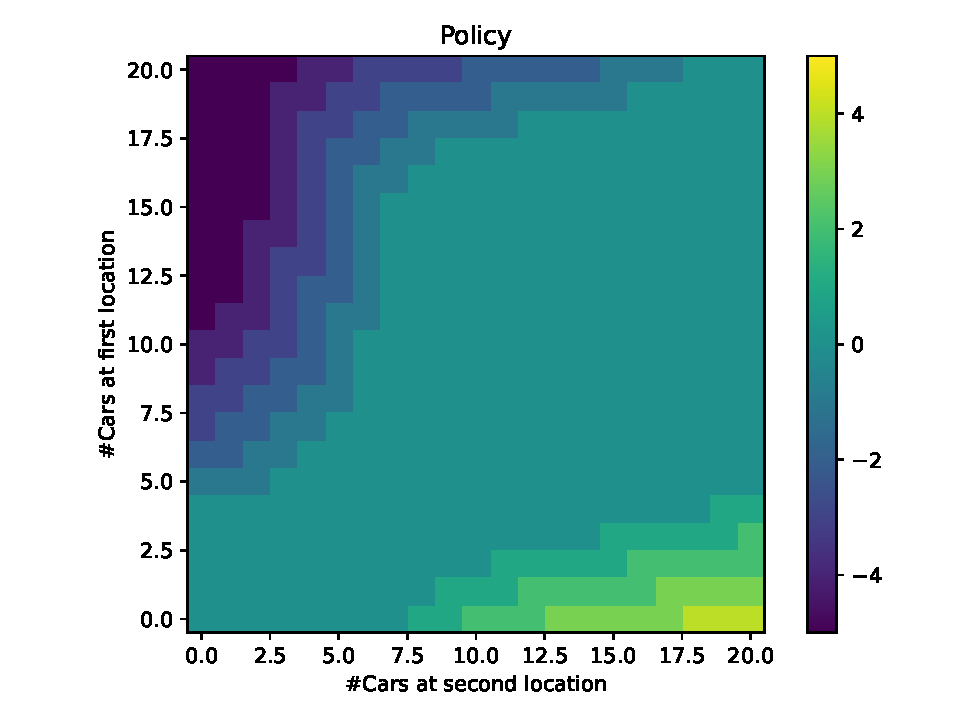
\includegraphics[width=0.8\textwidth]{chapters_latex/figures/ex_04_07_original.pdf}
    \caption{The original policy.}
\end{figure}

\begin{figure}[H]
    \centering
    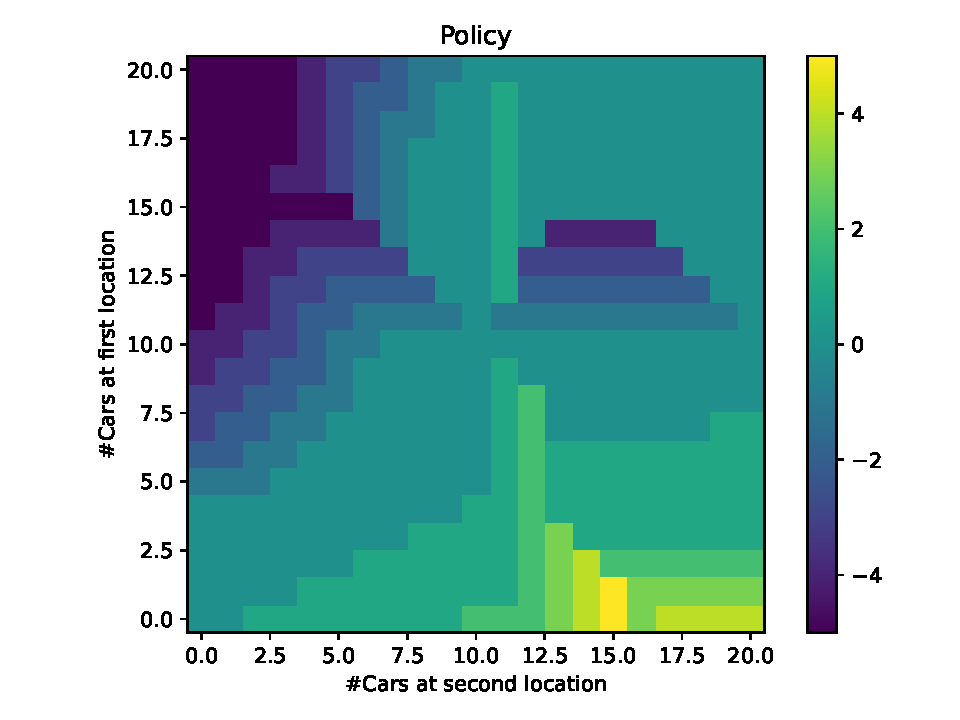
\includegraphics[width=0.8\textwidth]{chapters_latex/figures/ex_04_07_modified.pdf}
    \caption{The modified policy.}
\end{figure}

\subsection*{Exercise 4.8}
Why does the optimal policy for the gambler's problem have such a curious form? In particular, for capital of 50
it bets it all on one flip, but for capital of 51 it does not. Why is this a good policy? 

\subsubsection*{Solution:}

Betting 1 at 51 has two outcomes: receiving 1 coin with probability of 0.6 arriving at 52 coins, and losing 1 coin with probability of 0.4 arriving at 50 coins. At 50 coins we still have a relatively good chance of winning the game in one bet, and at 52 coins we have an even better chance. Betting more than one coin would mean that with great probability we would have less than 50 coins, in which case we would need a minimum of 2 bets to win the game, which is not good.

\subsection*{Exercise 4.9 (programming)}
Implement value iteration for the gambler's problem and
solve it for $p_h = 0.25$ and $p_h = 0.55$. In programming, you may find it convenient to
introduce two dummy states corresponding to termination with capital of 0 and 100,
giving them values of 0 and 1 respectively. Show your results graphically, as in Figure 4.3.
Are your results stable as $\theta \rightarrow 0$?

\subsubsection*{Solution:}

See the notebooks.

The state values for different head probabilities:

\begin{figure}[H]
    \centering
    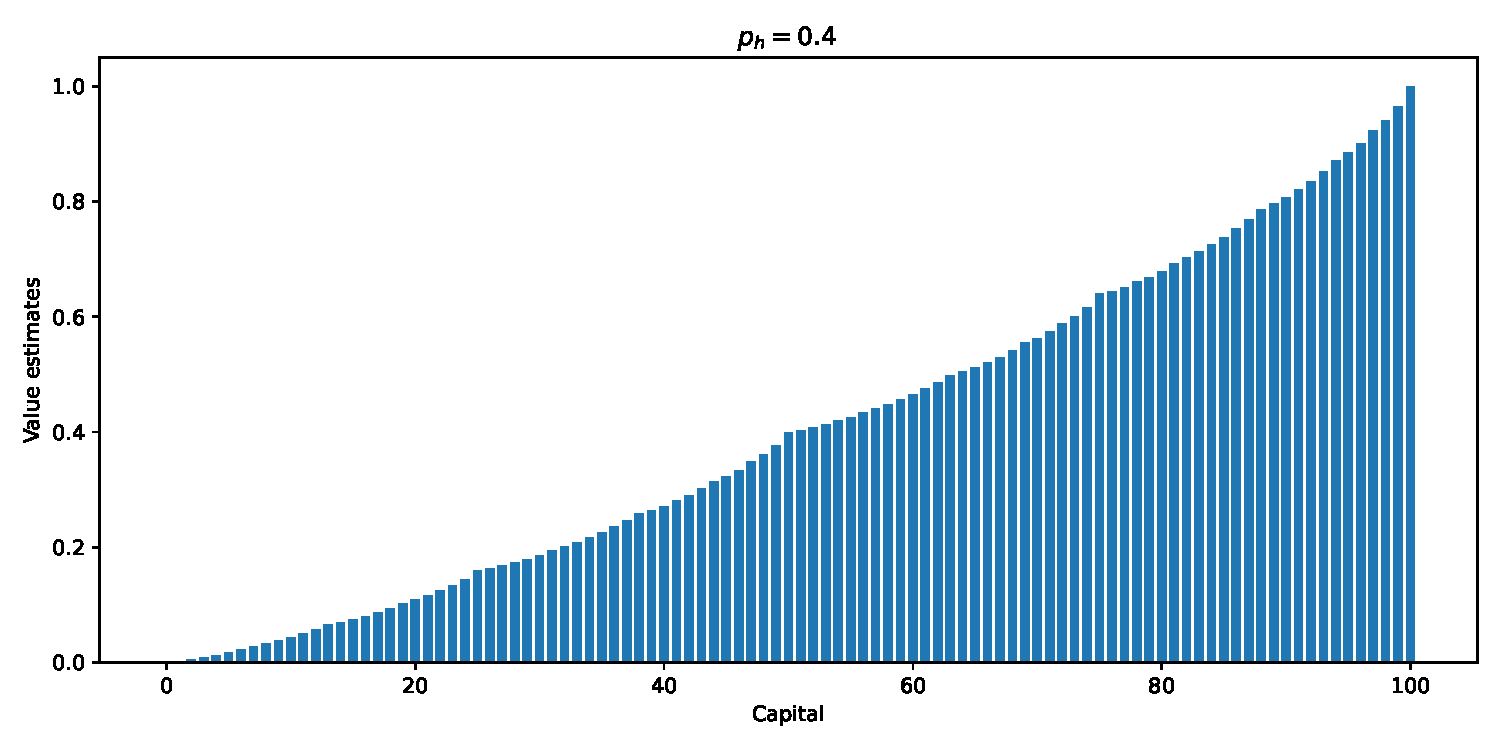
\includegraphics[width=0.8\textwidth]{chapters_latex/figures/ex_04_09_values_04.pdf}
\end{figure}

\begin{figure}[H]
    \centering
    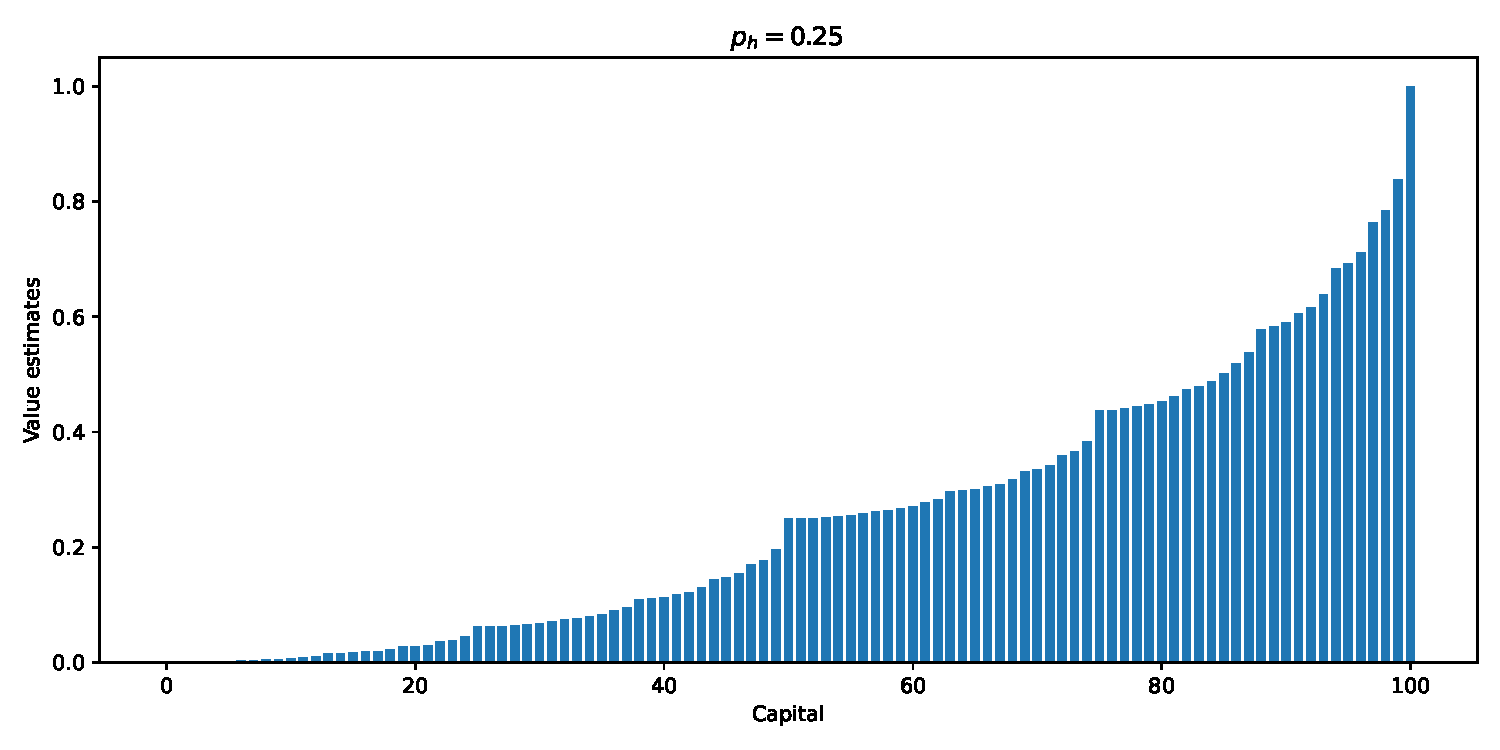
\includegraphics[width=0.8\textwidth]{chapters_latex/figures/ex_04_09_values_025.pdf}
\end{figure}

\begin{figure}[H]
    \centering
    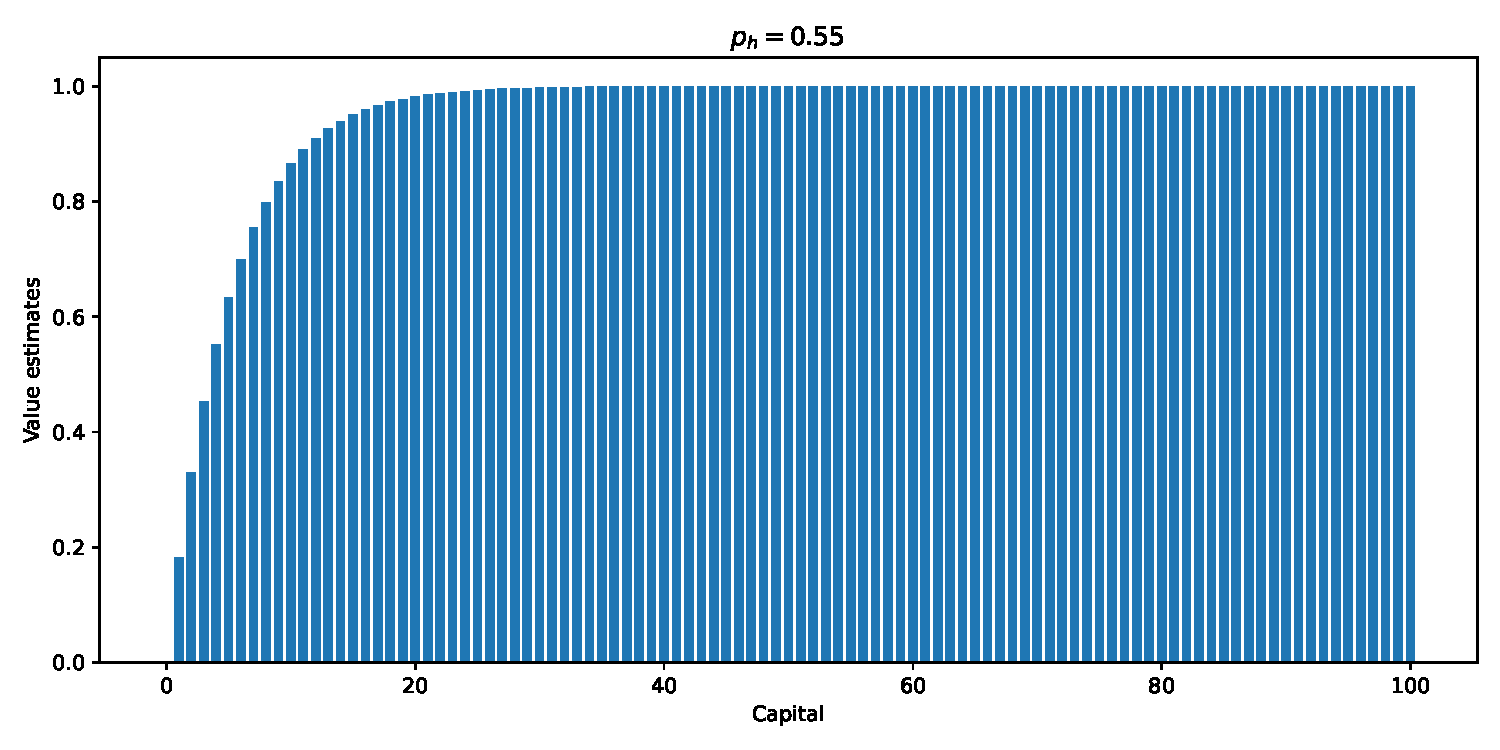
\includegraphics[width=0.8\textwidth]{chapters_latex/figures/ex_04_09_values_055.pdf}
\end{figure}

The optimal policies for different head probabilities:
\begin{figure}[H]
    \centering
    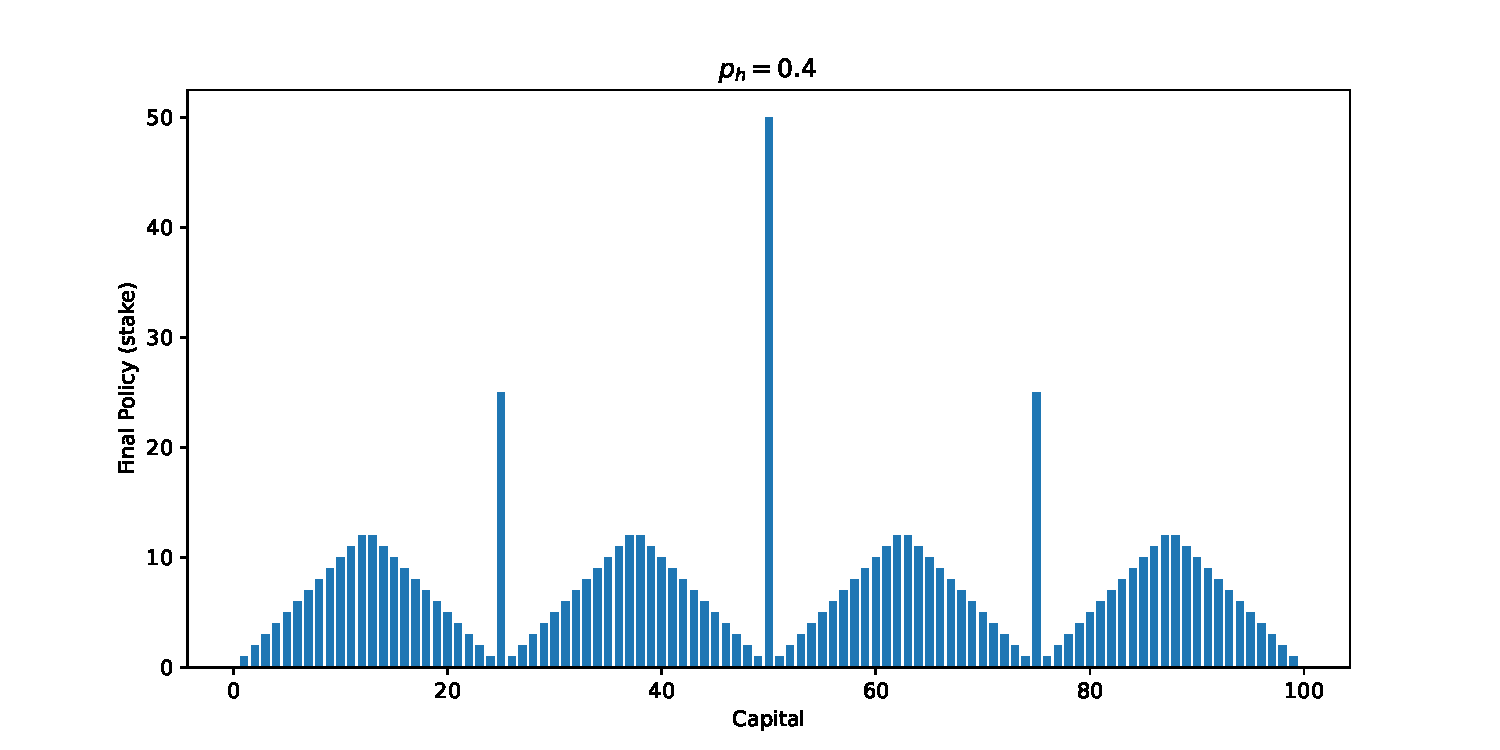
\includegraphics[width=0.8\textwidth]{chapters_latex/figures/ex_04_09_policies_04.pdf}
\end{figure}

\begin{figure}[H]
    \centering
    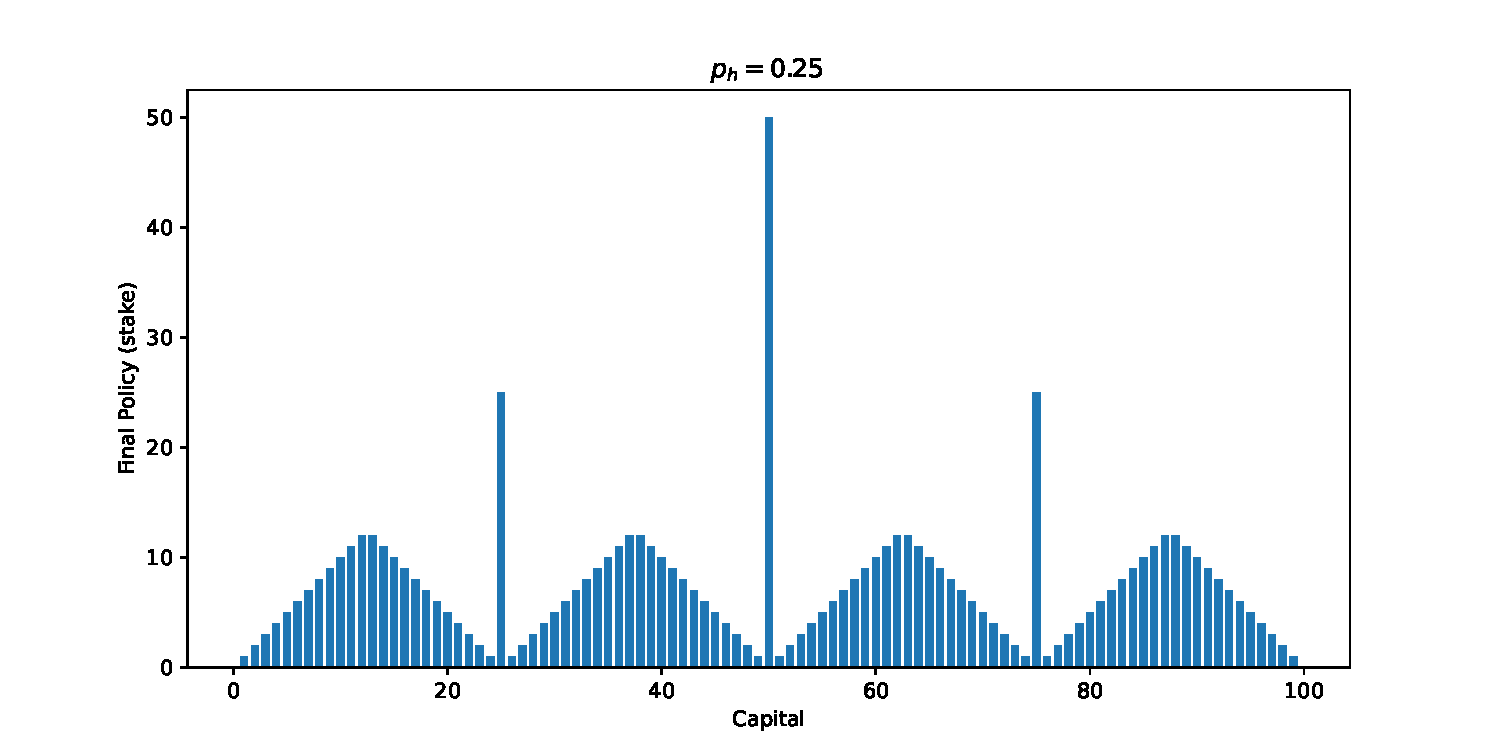
\includegraphics[width=0.8\textwidth]{chapters_latex/figures/ex_04_09_policies_025.pdf}
\end{figure}

\begin{figure}[H]
    \centering
    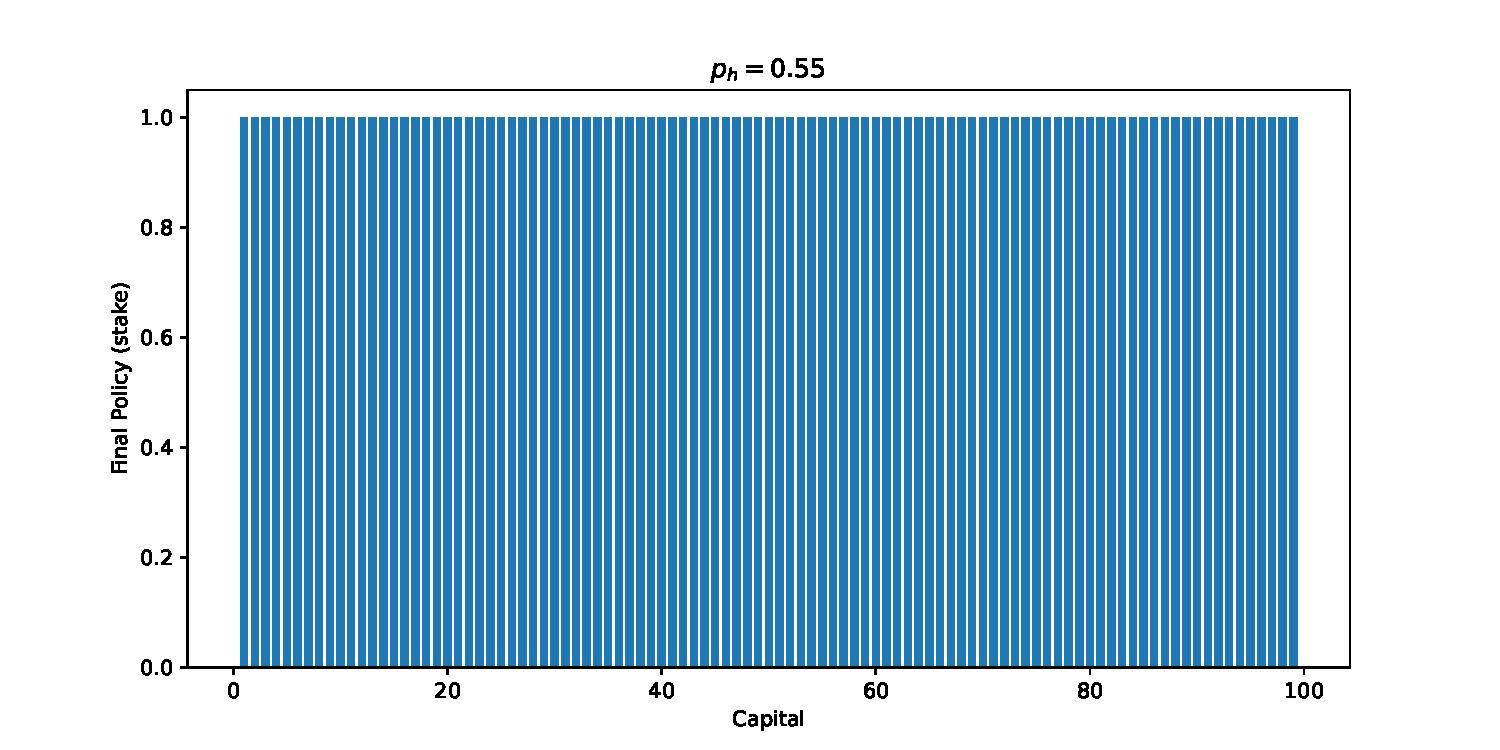
\includegraphics[width=0.8\textwidth]{chapters_latex/figures/ex_04_09_policies_055.pdf}
\end{figure}

\subsection*{Exercise 4.10}

What is the analog of the value iteration update (4.10) for action values,
$q_{k+1}(s,a)$?

\subsubsection*{Solution:}
\[
    q_{k+1}(s,a) = \sum_{s,r'} p(s',r \mid s, a) \left[r + \gamma \max_{a'} q_{k}(s',a') \right]
\]
\end{document}
